 % -*- root: ../main.tex -*-
\documentclass[../main.tex]{subfiles}
\begin{document}

\chapter{Les Glucocorticoïdes}

% =====================================================
% ======= BEGIN - Généralités

\section{Généralités}
Dans les années 1930, E. C. Kendall a mené des travaux critiques dans la compréhension de l'endocrinologie de la glande surrénale.
Il isola en effet plusieurs stéroïdes initialement dénommés "composés A, B, E, F", qui se révélèrent plus tard correspondre respectivement à la 11-déhydroxycorticostérone, à la \gls{cort}, au cortisol et à la cortisone.
Parallèlement, Wintersteiner et Reichstein contribuèrent jusqu'en 1953 à l'isolement de l'aldostérone.
D'après les premières expériences fonctionnelles menées sur les corticostéroïdes (hormones stéroïdes produites par la glande corticosurrénale), ils ont été classiquement séparés en deux catégories : les \glspl{mc} et les \glspl{gc} \citep{Simpson1952,Simpson1954}.
Les \glspl{mc} font partie intégrante du système rénine-angiotensine et ont été mis en évidence d'après leur capacité à stimuler la réabsorption de \gls{Na} dans les reins \citep{Gomez-Sanchez1996}.
Les \glspl{gc}, quant à eux, ont été définis initialement par leur capacité à stimuler la gluconéogenèse et leur action sur le métabolisme des carbohydrates (pour revue \citealp{McMahon1988}).
Ils ont cependant une action beaucoup plus générale dans la physiologie et l'homéostasie (\autoref{fig:gc-general-actions}).
En particulier, on leur reconnaît actuellement un rôle important au niveau du système cardiovasculaire et respiratoire, du \gls{snc}, de la peau, du foie, de la rate et des os.
De part leurs effets sur ces différents organes et tissus, il vont pouvoir affecter des processus aussi divers que le métabolisme général, la réponse au stress \citep{Sapolsky2000}, le système immunitaire et l'inflammation \citep{Busillo2013}, ou encore la régulation de processus circadiens \citep{Dickmeis2009}.

% BOTTOM caption
% ------------------------
\begin{figure}[!htbp]
\centering
\vspace{1\baselineskip}
\includegraphics[width=\textwidth]
% ------------------------
%
% SIDE caption
% ------------------------
%\begin{SCfigure}[\sidecaptionrelwidth][!htbp]
%\centering
%\vspace{1\baselineskip}
%\includegraphics[width=0.5\textwidth]
% ------------------------
%
% Main information
% ===========================================================
{Figures/gc-general-actions/gc-general-actions.pdf}
\caption[Principales fonctions biologiques impliquant les glucocorticoïdes]
{
Principales fonctions biologiques impliquant les \glspl{gc}.
a. Glande surrénale.
b. Poumons.
c. Coeur (et système cardiovasculaire).
d. Métabolisme squelettique.
e. Développement des muscles squelettiques.
f. Foie (fonctions hépathiques).
g. Rate.
h. Peau.
i. Système nerveux central (hypothalamus; hypophyse).
j. Métabolisme général.
k. Réponse au stress.
l. Système immunitaire et inflammation.
m. Cycles circadiens.
}
\label{fig:gc-general-actions}
% ===========================================================
%
% BOTTOM caption
% ------------------------
\end{figure}
% ------------------------
%
% SIDE caption
% ------------------------
%\end{SCfigure}
% ------------------------
%
%
%\missingfigure{Make a figure}

Au début des années 1970, plusieurs travaux ont convergé vers l'idée que les \glspl{gc} étaient liés dans le cytoplasme par des récepteurs spécifiques \citep{Baxter1971,Rousseau1972} et que leur action était médiée par la liaison à l'\gls{dna} pour réguler l'expression de gènes cibles \citep{Baxter1972,Payvar1981}.
L'action des \glspl{gr} médiée par la fixation au niveau de séquences régulatrices spécifiques fut démontrée par \citet{Chandler1983,Karin1984,Slater1985}
Le \gls{gr} a été initialement cloné par \citet{Weinberger1985}, tandis que le \glspl{mr} humain a été cloné par \citet{Arriza1987}.
Cependant, les deux catégories de corticosteroïdes ne sont pas restreintes à l'interaction avec leurs récepteurs respectifs et les \glspl{gc} peuvent avoir une activité \gls{mc} conséquente \citep{Funder1973,Reul1990}.

% -------------------------------
% +++ BEGIN - Les glandes surrénales

\subsection{Les glandes surrénales}
Les corticostéroïdes sont synthétisés par les glandes corticosurrénales.
Les surrénales sont des glandes asymétriques positionnées au dessus des reins (\autoref{fig:adrenal-gland}~A).
La circulation sanguine dans les surrénales est centripète.
Chaque couche est donc exposée à des concentrations croissantes en corticostéroïdes, ce qui est essentiel en particulier dans la \textit{medulla} qui nécessite des concentrations élevées de \gls{gc} afin de stimuler une des enzymes requises dans la synthèse d'adrénaline \citep{Nussey2001}.
Ces glandes sont composées de deux organes: la médullosurrénale et la corticosurrénale.

\begin{figure}[!htbp]
\centering
\vspace{1\baselineskip}
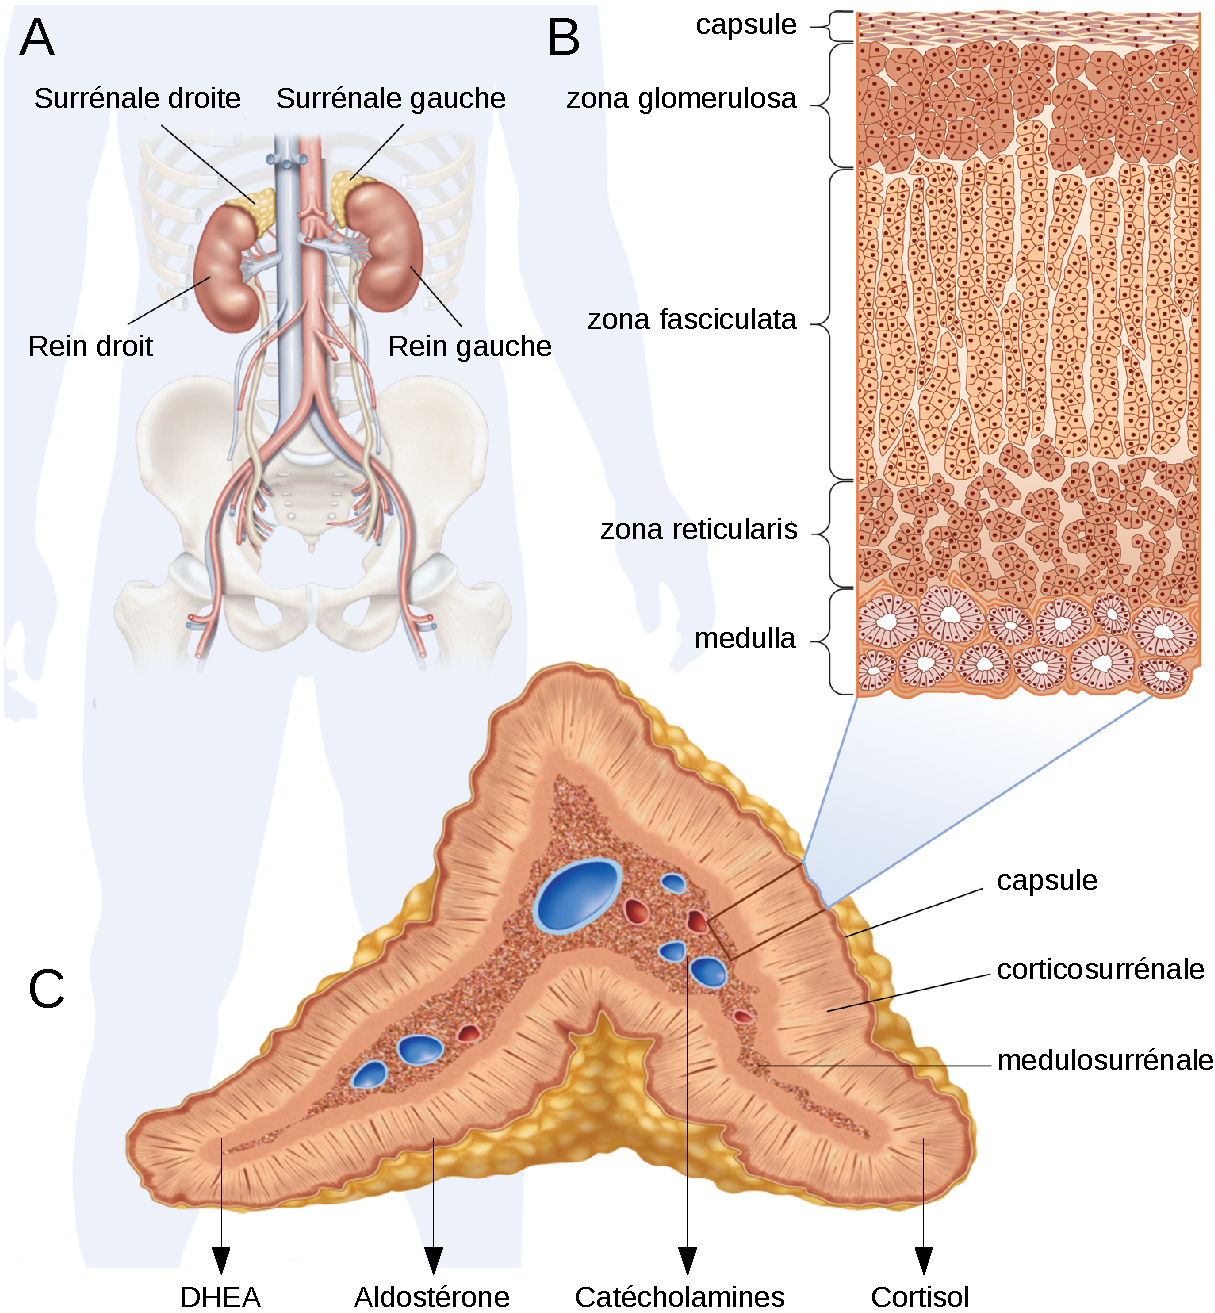
\includegraphics[width=\textwidth]
{Figures/adrenal-gland/adrenal-gland.pdf}
\caption[Les glandes surrénales]
{
Schéma des glandes surrénales.
Les glandes surrénales sont deux glandes situées au dessus des reins.
Elles sont entourées de la capsule, qui maintient leur structure.
La \textit{medulla} est la partie centrale des surrénales et compose les médullosurrénales.
C'est dans cette structure que les cellules chromaffines (en bleu) produisent les catécholamines sous forme d'adrénaline et de noradrénaline.
Le cortex compose les glandes corticosurrénales.
Il est subdivisé en trois couches, la \textit{zona glomerulosa} où sont produits les \glspl{mc}, la \textit{zona fasciculata} produisant essentiellement les \glspl{gc} et la \textit{zona reticularis} produisant essentiellement des hormones androgènes et une partie des \glspl{gc}.
Peu de stockage a lieu, et les hormones synthétisées sont immédiatement libérées dans la circulation sanguine.
Figure adaptée de Encyclopaedia Britannica.
}
\label{fig:adrenal-gland}
\end{figure}

\subsubsection{La corticosurrénale}
Dérivée du mésoderme \citep{Hammer2005}, elle est responsable de la production d'hormones stéroïdes non-sexuelles (essentiellement \glspl{gc}, \glspl{mc} et androstérone).
La corticosurrénale est composée de trois couches illustrées schématiquement \autoref{fig:adrenal-gland}~B \citep{Charlton1990,Parker1993} :
\begin{itemize}
\item La \textit{zona glomerulosa}, la couche la plus externe, positionnée juste sous la capsule.
C'est dans cette région qu'est synthétisée l'aldostérone dans le contexte du système rénine-angiotensine (\autoref{fig:adrenal-gland}~C).
Les \glspl{mc} sont en effet par ce biais, responsables du contrôle de la pression osmotique des fluides extracellulaires \citep{Feraco2013}.
\item La \textit{zona fasciculata}, dont les cellules sont organisées en fascicules. Les \glspl{gc} sont produits dans cette région sous forme de cortisol (\autoref{fig:adrenal-gland}~C) chez l'humain.
Cette région produit également une partie des précurseurs de stéroïdes androgènes sous forme de \gls{dhea}.
Cette dernière est convertie localement en \gls{dhea}-sulfate.
Ces précurseurs sont directement libérés dans la circulation afin d'être convertis en stéroides sexuels dans les gonades.
\item La \textit{zona reticularis} est la couche la plus interne de la corticosurrénale.
Elle est composée de cellules dont la configuration générale rappelle celle d'un réseau.
Une partie des \glspl{gc} sont synthétisés ici, ainsi qu'une partie de la \gls{dhea} et \gls{dhea}-sulfate (\autoref{fig:adrenal-gland}~C).
Pour revue voir \citep{McKay2003a}
\end{itemize}

\subsubsection{La médullosurrénale}
Composée de la \textit{medulla}, elle est dérivée du neuroectoderme et fait partie intégrante du \gls{sns}.
Elle est le lieu de production de catécholamines sous forme de 80 \% d'adrénaline et 20 \% de noradrénaline.
Celles-ci sont produites spécifiquement par les cellules chromaffines (tirant leur nom de leur coloration par des sels de chrome).
Les catécholamines sont dérivées de la tyrosine et sont les hormones principalement responsables de la réaction immédiate de lutte ou de fuite ("fight or flight response"), c'est à dire la réponse physiologique stéréotypée (mobilisation des réserves glucidiques, stimulation de la fonction cardiaque, dilatation des bronches et des vaisseaux sanguins ...) vers un effort physique intense dans le but de fuir ou d'affronter un danger imminent.

% +++ END - Les glandes surrénales
% -------------------------------

% ======= END - Généralités
% =====================================================

% :::::::::::::::::::::::::::::::::::::::::::::::::::::

% =====================================================
% ======= BEGIN - Métabolisme des GC

\section{Métabolisme et transport des glucocorticoïdes}

% -------------------------------
% +++ BEGIN - Synthèse des GC

\subsection{Synthèse des glucocorticoïdes}

\subsubsection{Stéroïdogenèse et biosynthèse des GC}
Toutes les hormones stéroïdes sont des dérivés du cholestérol, un stérol (molécule organique) identifié pour la première fois par François Poulletier de la Salle en 1769.
C'est un composé présent chez les métazoaires permettant de réguler physiquement la perméabilité et la fluidité des membranes cellulaires en fonction de la température \citep{Cooper1978}.
Le cholestérol est produit \textit{de novo} par toutes les cellules, en particulier dans le foie, les intestins, les gonades et les surrénales, mais peut être obtenu par l'alimentation.
\par
%Sa synthèse est effectuée à partir d'acétyl-\gls{coa} et d'acétoacétyl-\gls{coa} qui sont hydratées en \gls{hmg}-\gls{coa}.
%La réduction de l'\gls{hmg}-\gls{coa} en mevalonate est l'étape limitante et irréversible de la biosynthèse du cholestérol.
%Plusieurs étapes supplémentaires \gls{atp}-dépendantes sont ensuite nécessaire pour convertir le mavelonate en 3-isopentenyl pyrophosphate.
%Trois molécule de 3-isopentenyl pyrophosphate sont condensées en farnesyl pyrophosphate, 2 molécules de ce dernier sont condensées en squalène qui sera cyclisé.
%Le lanostérol obtenu est ensuite converti en choléstérol.
%Le cholestérol est transporté dans la circulation sanguine par des lipoprotéines (les \glspl{ldl}, \glspl{hdl} et \glspl{vldl}).
%
%% ONE columns
% ------------------------
%\begin{figure}[!htbp]
%\centering
%\includegraphics[width=\textwidth]
% ------------------------
%
% TWO columns
% ------------------------
\begin{SCfigure}[\sidecaptionrelwidth][!htbp]
\centering
\includegraphics[width=0.5\textwidth]
% ------------------------
%
% Main information
% ===========================================================
{Figures/cholesterol/cholesterol.pdf}
\caption[Cholestérol]
{
Une molécule de cholestérol est modifiée par des enzymes spécialisées catalysant la conversion du 3-hydroxyl en cétone, l'isomérisation de la double liaison C5-C6 en C4-C5 et l'attaque des carbones C11, et C16 à C21.
}
\label{fig:cholesterol}
% ===========================================================
%
% ONE columns
% ------------------------
%\end{figure}
% ------------------------
%
% TWO columns
% ------------------------
\end{SCfigure}
% ------------------------
%
%
%\missingfigure{Make a figure}

La biosynthèse des \glspl{gc} fait intervenir plusieurs enzymes qui modifient une molécule de cholestérol ou de dérivé du cholestérol.
Les \glspl{gc}, sous forme de cortisol ou \gls{cort}, sont obtenus en étapes successives détaillées dans la \autoref{fig:steroidogenesis}.
La chaîne latérale du cholestérol est d'abord clivée par la \gls{p450scc} \citep{Chung1986}, pour obtenir de la pregnénolone.
Celle-ci peut être convertie en \gls{17aohpreg}, \gls{17aohprog} ou en progestérone par le biais de la gls{3bhsd} et de la \gls{17aohase}.
La \gls{17aohprog} et la progestérone sont ensuite hydroxylées successivement par la \glspl{21ohase}, formant ainsi le 11-déoxycortisol et la \gls{doc}, et la \gls{11bohase} pour donner le cortisol et la \gls{cort}.
L'aldostérone peut être formée à partir de cette dernière par la \gls{18bohase}.
Pour revue, voir \citep{Ghayee2007}

\begin{figure}[!htbp]
\centering
\vspace{1\baselineskip}
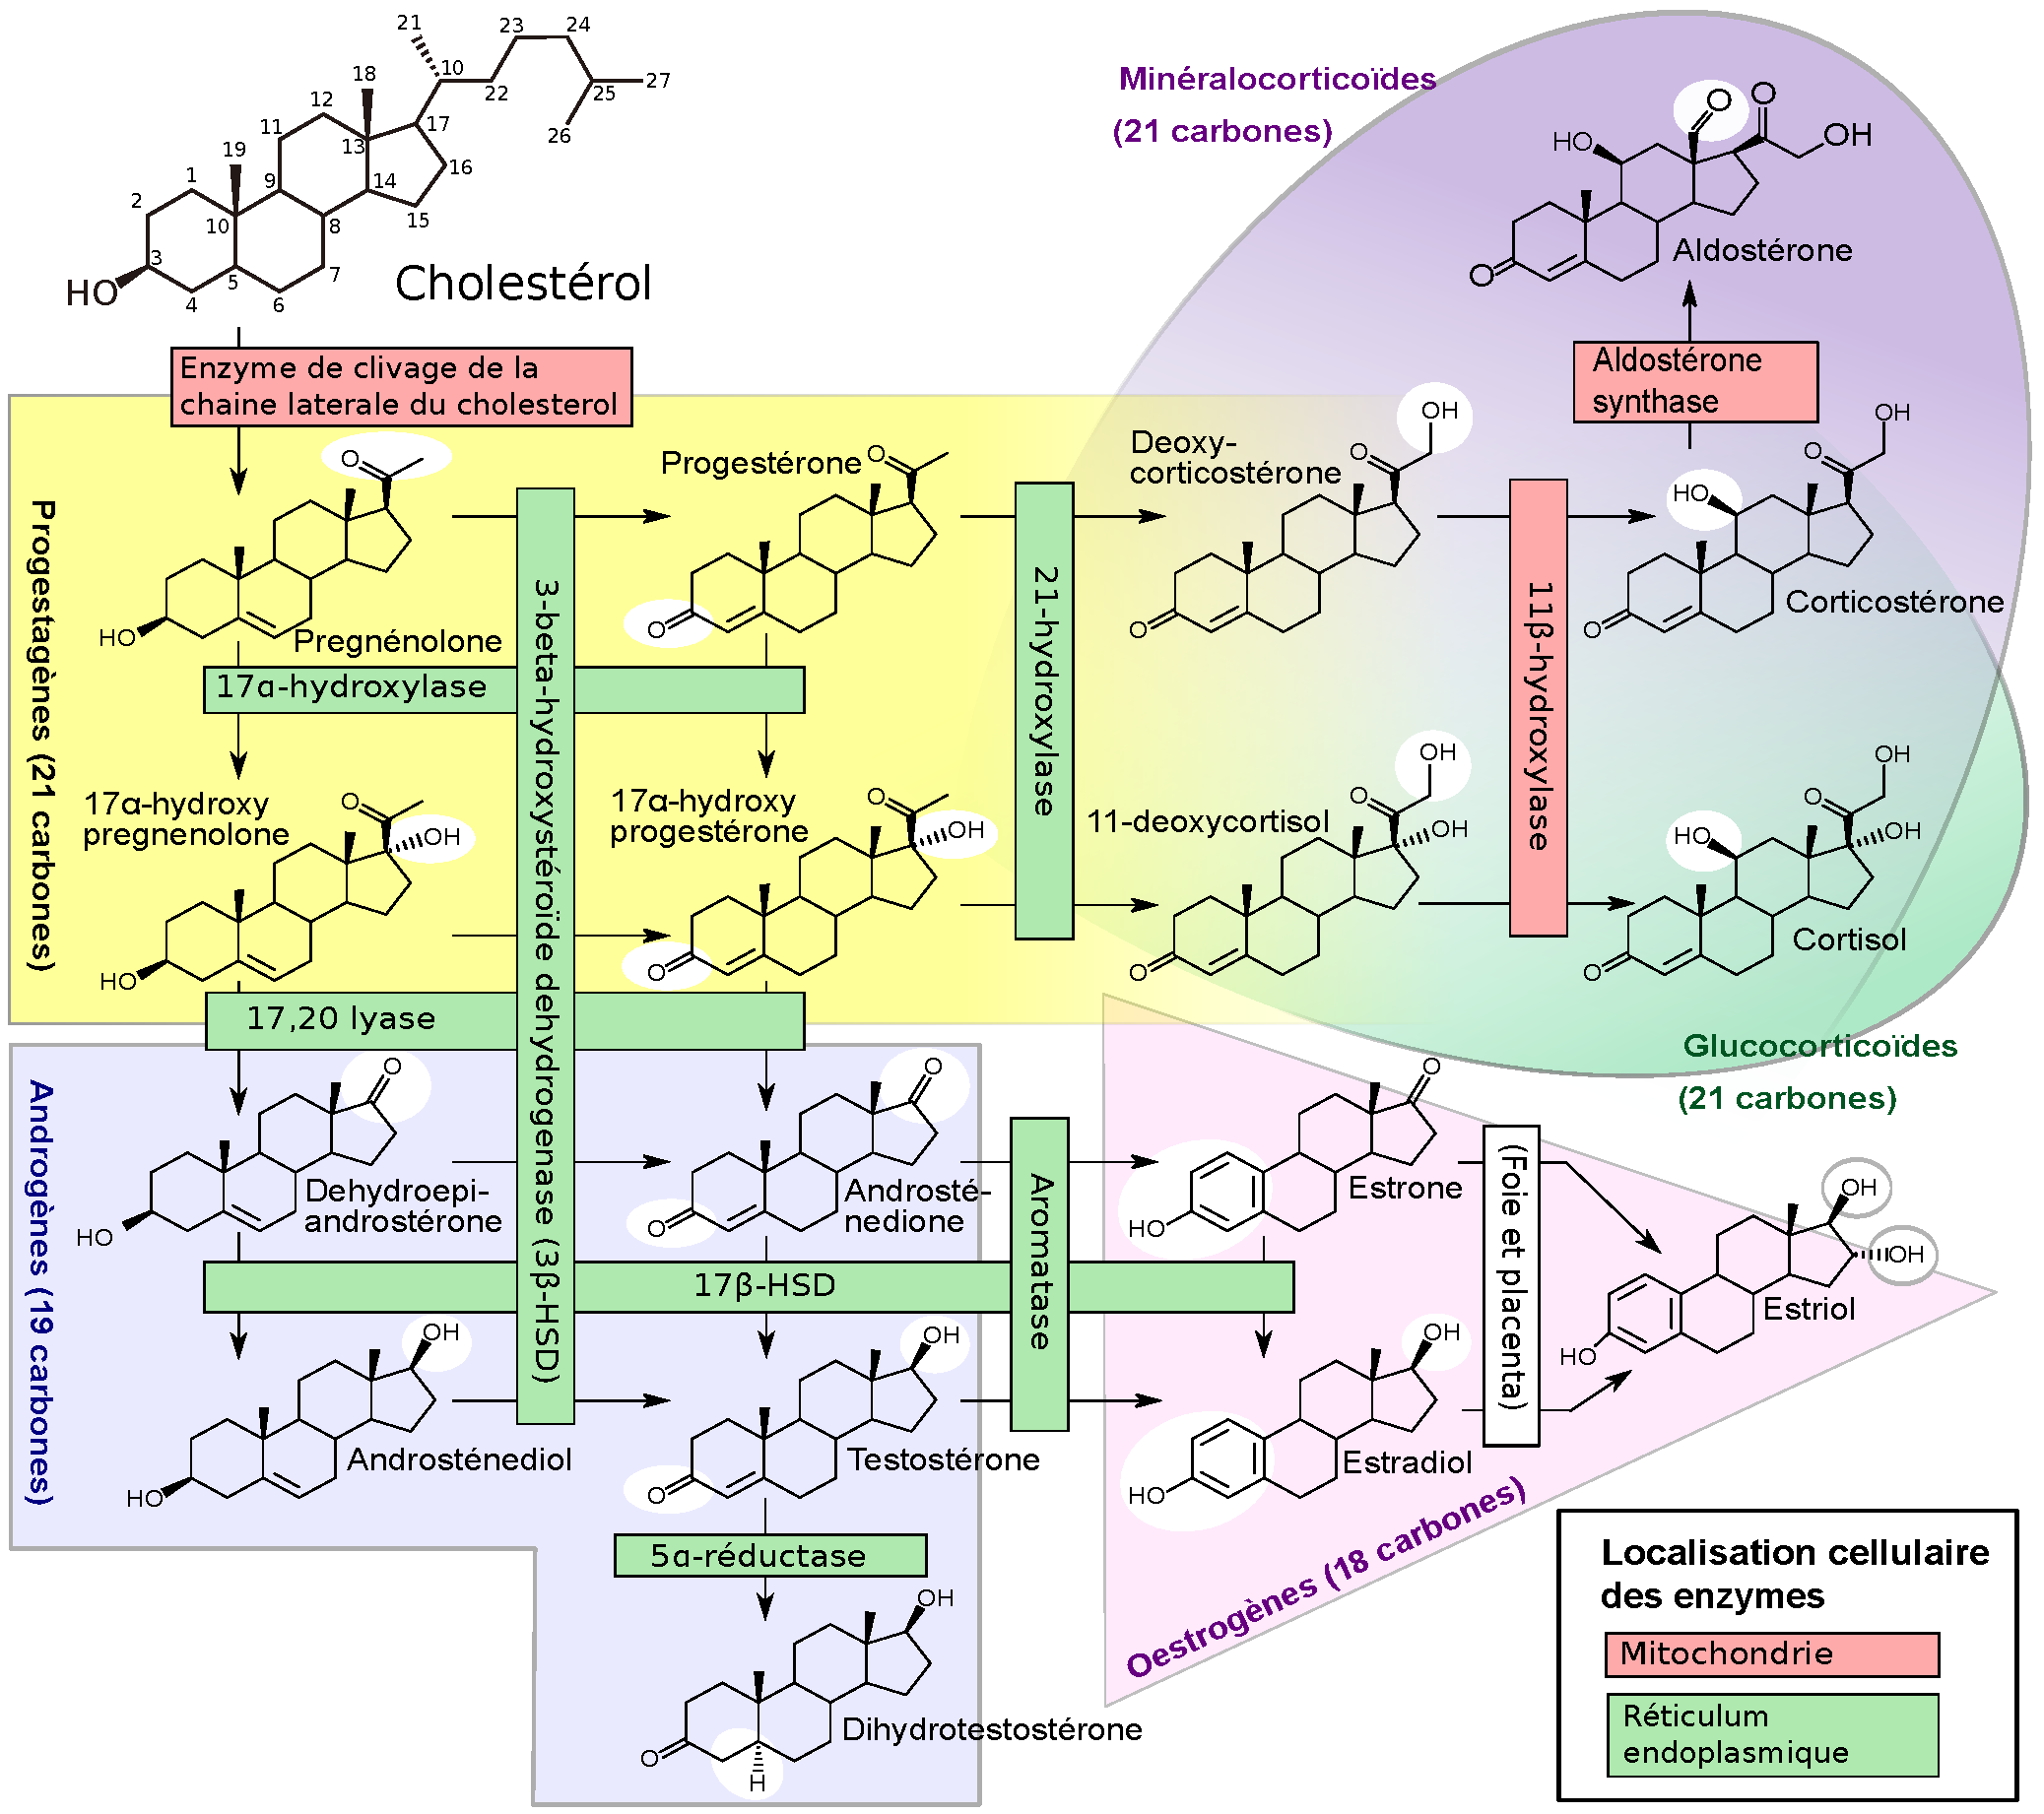
\includegraphics[width=\textwidth]
{Figures/steroidogenesis/steroidogenesis.pdf}
\caption[Principales étapes de la stéroidogenèse]
{
\glsreset{doc}\glsreset{cort}
Principales étapes de la stéroïdogenèse.
Le choléstérol est tout d'abord convertit en pregnénolone, qui à son tour est convertie en \gls{17aohpreg}, en \gls{17aohprog} ou en progestérone.
Ces deux dernières servent de précurseurs directs à l'obtention de 11-déoxycortisol et de \gls{doc}.
Enfin, par hydroxylation du 11-déoxycortisol et de la \gls{doc}, le cortisol et la \gls{cort} sont obtenus.
Les stéroïdes sexuels sont synthétisés à partir de \gls{17aohpreg} et de \gls{17aohprog} (partie inférieure du diagramme).
Tiré de "Steroidogenesis.svg" par David Richfield et Mikael Häggström.
}
\label{fig:steroidogenesis}
\end{figure}

\subsubsection[Axe hypothalamo-hypophyso-adrénal]{Axe hypothalamo-hypophyso-adrénal}
La sécrétion de cortisol est contrôlée par l'axe \gls{hpa} faisant intervenir le \gls{snc} et la corticosurrénale (\autoref{fig:hpa}; \citealp{Herman1997}).
La production de \glspl{gc} suit un rythme circadien imposé en partie par l'axe \gls{hpa}, avec chez les mammifères diurnes un pic de \glspl{gc} circulants au réveil (\citealp{Dickmeis2009} pour revue).
Cette production de \glspl{gc} active des neurones corticotrophes dans l'anté-hypophyse et stimule la libération d'\gls{acth} dans la circulation sanguine.
L'\gls{acth} agit ensuite sur la corticosurrénale pour induire la production de cortisol.
Enfin, le cortisol (la \gls{cort} chez les rongeurs, les sauropsides et les amphibiens) agit sur l'hypothalamus et l'anté-hypophyse pour exercer un rétrocontrôle négatif sur la sécrétion de \gls{crh} et d'\gls{acth}.
Parallèlement, le cortisol et les autres hormones stéroïdes agissent sur leurs tissus cibles pour médier la réponse à un stress \citep{Herman1997,Tsigos2002}.
\par
Une production accrue de \glspl{gc} peut également avoir pour origine un stress :
Un stress induit la production de \gls{crh} par l'hypothalamus, stimulant la production de \glspl{gc} \textit{via} cet axe.

% BOTTOM caption
% ------------------------
\begin{figure}[!htbp]
\centering
\vspace{1\baselineskip}
\includegraphics[width=\textwidth]
% ------------------------
%
% SIDE caption
% ------------------------
%\begin{SCfigure}[\sidecaptionrelwidth][!htbp]
%\centering
%\vspace{1\baselineskip}
%\includegraphics[width=0.5\textwidth]
% ------------------------
%
% Main information
% ===========================================================
{Figures/hpa/hpa.pdf}
\caption[Axe hypothalamo-hypophyso-adrénal]
{
L'axe \gls{hpa} implique l'hypothalamus, l'anté-hypophyse et les glandes corticosurrénales.
L'hypothalamus secrète la \gls{crh}, qui à son tour stimule la production d'\gls{acth} par l'hypophyse.
L'\gls{acth} libérée dans la circulation sanguine va pouvoir agir sur la glande corticosurrénale pour initier la synthèse de corticostéroïdes (quasiment aucun stockage n'a lieu).
Ceux-ci vont enfin agir d'une part sur les tissus cibles pour maintenir la physiologie de base, et d'autre part sur l'hypothalamus pour exercer un rétrocontrôle négatif sur la production de \gls{crh}.
Un stress peut également être à l'origine d'une élévation de la concentration en \glspl{gc} \textit{via} la stimulation de la production de \gls{crh}.
Dans ce cas, l'action des \glspl{gc} sur les tissus cibles va induire un maintien de l'homéostasie en contribuant à moduler la réponse au stress.
}
\label{fig:hpa}
% ===========================================================
%
% BOTTOM caption
% ------------------------
\end{figure}
% ------------------------
%
% SIDE caption
% ------------------------
%\end{SCfigure}
% ------------------------
%
%
%\missingfigure{Make a figure}

% +++ END - Synthèse des GC
% -------------------------------
% +++ BEGIN - Transport des GC

\subsection{Transport des glucocorticoïdes}
Les corticostéroïdes, comme d'autres hormones stéroïdes, sont couplés à une protéine de transport dans le sang, la \gls{cbg} \citep{Rosner1990}.
C'est une $\alpha$-globuline produite dans le foie capable de lier les \glspl{gc} et présentant de fortes similarités de séquence avec les serpines.
Une fraction élevée des hormones stéroïdes circulantes est liée à la \gls{cbg} \citep{Bittar1997,Becker2001}:
\begin{itemize}
\item Environs 3/4 du cortisol et de la cortisone circulants
\item la majeur partie de la \gls{cort} et de la \gls{doc}.
\item Environs 1/6 de l'aldostérone. La moité est liée à l'albumine et le reste est sous forme libre.
\item Une fraction minoritaire de la progestérone (environs 1/6)
\end{itemize}

% +++ END - Transport des GC
% -------------------------------
% +++ BEGIN - Métabolisme local des GC

\subsection{Métabolisme local des glucocorticoïdes}\label{subsec:local-gc-metabo}
De même que pour les \glspl{ht}, les \glspl{gc} sont métabolisés en formes plus ou moins actives au niveau des tissus cibles, offrant ainsi un mécanisme de régulation supplémentaire de leur action systémique.
Les enzymes clés du métabolisme local des \glspl{gc} sont la \gls{11bhsd1} \glsunset{11bhsd2} et la \gls{11bhsd2}, qui assurent l'inter-conversion (observée dès les années 1950) de \glspl{gc} actifs (cortisol ou \gls{cort}) et de formes inertes (cortisone ou 11-déhydrocorticostérone).
Ça n'est que dans les années 1980 que leur importance physiologique fut prise en compte \citep{Edwards1988,Funder1988} et permit de résoudre le paradoxe des interactions croisées entre \glspl{mc} et \glspl{gc}.
En effet, la présence de la \gls{11bhsd2} dans les tissus cibles des \glspl{mc} inactive rapidement les \glspl{gc} permettant l'accès sélectif de l'aldostérone aux \glspl{mr} (\autoref{fig:11bhsd}, voir pour revue \citealp{Seckl2001}).

% BOTTOM caption
% ------------------------
\begin{figure}[!htbp]
\centering
\vspace{1\baselineskip}
\includegraphics[width=\textwidth]
% ------------------------
%
% SIDE caption
% ------------------------
%\begin{SCfigure}[\sidecaptionrelwidth][!htbp]
%\centering
%\vspace{1\baselineskip}
%\includegraphics[width=0.5\textwidth]
% ------------------------
%
% Main information
% ===========================================================
{Figures/11bhsd/11bhsd.pdf}
\caption[Rôles des 11-$\beta$-HSDs dans le métabolisme local des glucocorticoïdes]
{
La \gls{11bhsd2} agit dans les tissus cibles des \glspl{mc} pour empêcher le cortisol de lier aspécifiquement les \glspl{mr}.
La \gls{11bhsd1}, quant à elle, agit dans de nombreux tissus pour augmenter la concentration locale en \glspl{gc} et ainsi maintenir l'exposition des \glspl{gr} à leurs ligands.
Tiré de \citet{Seckl2001}.
}
\label{fig:11bhsd}
% ===========================================================
%
% BOTTOM caption
% ------------------------
\end{figure}
% ------------------------
%
% SIDE caption
% ------------------------
%\end{SCfigure}
% ------------------------
%
%
%\missingfigure{Make a figure}

De façon intéressante, la \gls{11bhsd2} est une déshydrogénase stricte.
Au contraire, la \gls{11bhsd2} possède principalement une activité réductase, mais peut sous certaines conditions prendre le rôle d'une 11-$\beta$-déshydrogénoase et agir ainsi en tant qu'enzyme inactivante des \glspl{gc} \citep{Phillips1989}.

% +++ END - Métabolisme local des GC
% -------------------------------

% ======= END - Métabolisme des GC
% =====================================================
% :::::::::::::::::::::::::::::::::::::::::::::::::::::

% =====================================================
% ======= BEGIN - Roles des GC

\section{Rôles des glucocorticoïdes}

% -------------------------------
% +++ BEGIN - Rôles Développementaux

\subsection{Rôles Développementaux}
Les \glspl{gc} ont de nombreux rôles développementaux et dans l'organogenèse.
La signalisation des \glspl{gc} est en effet impliquée dans la maturation et l'activation fonctionnelle de nombreux organes dont le coeur, les poumons, les intestins, le pancréas et les reins \citep{Majumdar1985,Liggins1994,Pierce1995,Gesina2004}.
Les \glspl{gc} de synthèse sont ainsi devenus un outil médical important pour aider le développement des organes chez les nouveaux-nés prématurés, en particulier la maturation des poumons \citep{Becker2001} en stimulant la production de surfactant \citep{Bolt2001}.
Chez la souris, l'inactivation du gène codant pour \gls{gr} empêche le développement des poumons \citep{Cole2001}.
Dans le cadre du développement du système digestif, les \glspl{gc} régulent la communication cellulaire dans l'intestin grêle \citep{Schaeffer2000}.
Les \glspl{gc} ont enfin de profonds effets sur le développement squelettique en augmentant l'activité des ostéoblastes et des effets délétères sur le développement cérébral en retardant la maturation des neurones et des cellules gliales.
De façon intéressante, chez les mammifères, l'incapacité de certaines structures cérébrales comme l'hippocampe à répondre au signal \gls{gc} à cause d'une expression ou d'une activité altérée de \gls{gr} a été associée à certain comportements pathologiques \citep{Liu1997,McGowan2009,Zhang2013}.
Ceci suggère que, jusqu'à un certain point, les \glspl{gc} pourraient participer au modelage du comportement d'un organisme en réponse à un environnement adverse.
\par
Les détails de l'action des \glspl{gc} dans l'organogenèse et les facteurs de transcription et morphogènes sous le contrôle des \glspl{gc} sont toutefois encore mal connus.

% +++ END - Rôles Développementaux
% -------------------------------
% +++ BEGIN - Actions sur les fluides extra-cellulaires

\subsection{Actions sur les fluides extra-cellulaires}
Bien que l'action des corticostéroïdes sur les fluides extra-cellulaires et leur concentration ionique soit majoritairement assurée par les \glspl{mc}, les \glspl{gc} y participent également \citep{McKay2003}.
Leurs actions sur les reins diffèrent de celles des \glspl{mc} par l'absence d'excrétion d'hydrogène.
Ils participent toutefois à l'augmentation de la diurèse, de la filtration glomérulaire, ainsi qu'à la rétention de \gls{Na} et l'excrétion de \gls{K}.
Des pathologies associées à des taux élevés en \glspl{gc} sont la néphrocalcinose et la néphrolithiase.

% +++ END - Actions sur les fluides extra-cellulaires
% -------------------------------
% +++ BEGIN - Rôles dans le système immunitataire

\subsection{Rôles dans le système immunitaire}\label{subsec:gc-immune}
Dans un contexte médical, les \glspl{gc} ont vite représenté des cibles thérapeutiques importantes à cause de leurs puissants effets anti-inflammatoires.
Toutefois, il est réducteur de ne voir chez les \glspl{gc} que ce type d'action.
Les \glspl{gc} sont plutôt en réalité un rhéostat cellulaire qui assure une réponse adaptée du système immun.
Les \glspl{gc} affectent ainsi toutes les phases de la réponse immunitaire et en agissant à cinq niveaux (pour revue, voir \citealp{Busillo2013}) :
Ils augmentent l'expression de facteurs contrôlant le système immunitaire inné et inhibent l'expression de cytokines pro-inflammatoires en bloquant l'action de facteurs modulant l'aspect acquis du système immunitaire, notamment \textit{via} \gls{ap1}, \gls{nfkb}.
Enfin, les \glspl{gc} ont la capacité de promouvoir la résolution de l'inflammation (c'est à dire le retour à un état non-inflammatoire) et la restauration de l'homéostasie en stimulant la sécrétion de molécules pro-résolutives (comme Annexin-1, favorisant ) et en entraînant l'apoptose des cellules T et des neutrophiles \citep{Parrillo1979}.
Parallèlement, les \glspl{gc} induisent un phénotype anti-inflammatoire chez certains macrophages et stimulent la prise en charge des cellules apoptotiques.
\par
Outre leurs effets anti-inflammatoires bien décrits, il semblerait que les \glspl{gc} puissent également avoir une action pro-inflammatoire en exacerbant la réponse aux lipopolysaccharides \citep{Munhoz2010,Frank2012}, et agissant en synergie avec la signalisation \gls{tnfa} \citep{Lannan2012}.

% +++ END - Rôles dans le système immunitaire
% -------------------------------
% +++ BEGIN - Rôles dans la réponse au stress

\subsection{Rôles dans l'homéostasie et la réponse au stress}\label{subsec:gc-role-stress}
La notion de stress est centrale lorsque l'on mentionne les actions des \glspl{gc}.
On peut même aller plus loin et considérer que leurs effets diversifiés sur le développement, le métabolisme, le comportement, et le système immunitaire constituent plusieurs facettes de la réponse d'un vertébré face à un environnement hostile.
Le terme de stress dans un contexte biologique est né notamment grâce à Walter Bradford Cannon et Hans Selye.
Le premier caractérisa la réponse de lutte ou de fuite ("fight-or-flight response"; \citealp{Cannon1915}) et développa le concept d'homéostasie en 1932 à partir des travaux de Claude Bernard.
Le second conceptualisa le stress comme intégrant deux composantes:
un ensemble de réponses stéréotypées, le \gls{gas}, et le développement d'un état pathologique découlant d'un stress continu et non-soulagé \citep{Selye1946}.
Ainsi, la réponse de l'organisme est double, et fait intervenir des mécanismes différents visant à faire face au stress à court terme et à long terme.

% BOTTOM caption
% ------------------------
\begin{figure}[!htbp]
\centering
\vspace{1\baselineskip}
\includegraphics[width=\textwidth]
% ------------------------
%
% SIDE caption
% ------------------------
%\begin{SCfigure}[\sidecaptionrelwidth][!htbp]
%\centering
%\vspace{1\baselineskip}
%\includegraphics[width=0.5\textwidth]
% ------------------------
%
% Main information
% ===========================================================
{Figures/stress-response/stress-response.pdf}
\caption[Réponses physiologiques au stress]
{
Réponses physiologiques à court et à long terme à un stress.
Dés les premières minutes, la médullosurrénale est stimulée via le système nerveux sympathique et sécrète des catécholamines responsables de l'augmentation et de l'alimentation de comportement de confrontation ou de fuite (A).
À plus long terme (quelques heures à plusieurs jours), les corticostéroïdes provoquent un changement de la physiologie du système circulatoire et excrétoire et participent à l'installation d'un état physiologique correspondant à la réaction de résistance (B).
Les \glspl{gc} induisent la majorité de la réponse au stress en augmentant la mobilisation des ressources énergétiques et en supprimant le système immun.
D'autres organes endocrines jouent un rôle, notamment le foie (augmentation de la glycémie sanguine) et la thyroïde (augmentation du catabolisme et de la production d'énergie à partir des stocks mobilisés).
}
\label{fig:stress-response}
% ===========================================================
%
% BOTTOM caption
% ------------------------
\end{figure}
% ------------------------
%
% SIDE caption
% ------------------------
%\end{SCfigure}
% ------------------------
%
%
%\missingfigure{Make a figure}

Dans un premier temps, le \gls{sns} est immédiatement impliqué avec la stimulation directe de la medullosurrénale à sécréter des catécholamines responsables du comportement de lutte ou de fuite (\autoref{fig:stress-response}~A).
\par
Dans un second temps (\autoref{fig:stress-response}~B), la médiation de la réponse passe par les \glspl{gc} et les \glspl{mc} et vise à modifier la physiologie de façon à résister à un stress prolongé.
En particulier, les \glspl{mc}, via le système rénine-angiotensine, vont augmenter le volume sanguin et la pression artérielle.
Les \glspl{gc} vont, quant à eux, induire une transition métabolique (pour revue \citealp{Munck2010,Weissman1990}) ayant pour conséquence la consommation des stocks de lipides et protéines \citep{Richard1993}, l'augmentation de la glycémie sanguine par glycogénolyse et gluconéogenèse \citep{Eigler1979}, ou encore la suppression du système immunitaire (voir \autoref{subsec:gc-immune}).
Faire face à un stress prolongé va également inclure la participation d'autres organes endocrines, notamment le foie, qui via les \glspl{igf} et \gls{pepck}, augmente le métabolisme glucidique \citep{Exton1987,Weissman1990}, et la thyroïde, qui via les \glspl{ht}, augmente le catabolisme du glucose \citep{Weissman1990}.
\par
Dans une optique plus générale, les \glspl{gc} peuvent être vus non pas comme l'agent qui suscitera la réponse au stress, mais plutôt comme celui qui modulera la réponse au stress pour éviter un emballement de la réponse physiologique dans un premier temps (action modulatrice, se manifestant au bout d'une à quelques heures), puis qui préparera l'organisme à des stress ultérieurs (action préparatrice, se manifestant au bout de quelques heures et perdurant jusqu'à plusieurs jours) \citet{Sapolsky2000}.
\par
Les actions modulatrices et préparatrices des \glspl{gc} peuvent toutes deux se subdiviser en trois catégories :
\begin{itemize}
\item Les actions permissives. Exercées par les \glspl{gc} indépendamment de l'augmentation de leur concentration, elles font partie des actions basales des \glspl{gc}.
Ceci n'exclut cependant pas leur participation lors de la première exposition à un stress.
\item Les actions suppressives. Elles visent à refréner les réactions de défense induites par la réponse au stress, et sont dépendantes d'une augmentation de la quantité de \glspl{gc}.
\item les actions stimulatrices. À l'opposé des actions suppressives, elles visent à augmenter et stimuler la réponse au stress de la première vague de réponse.
Ces actions dépendent également d'une augmentation de la quantité de \glspl{gc}.
\end{itemize}
Les actions préparatrices peuvent, au même titre que les actions modulatrices, aider ou prévenir la réponse au stress selon les trois modalités listées au paragraphe précédent.
Elles n'affectent cependant pas la réponse immédiate, et préparent l'organisme sur le long terme pour faire face à l'exposition répétée à un stress.
\par
Plusieurs critères ont été établis afin de déterminer à quelle catégorie une action particulière des \glspl{gc} peut être attribuée.
Ils sont basés sur quatre paramètres:
\begin{itemize}
\item Le critère de conformité (augmentation ou suppression de l'effet des hormones impliquées dans la première vague de réponse)
\item le critère de temporalité (effet manifesté quelques minutes, heures ou jours après l'exposition au stress)
\item le critère de soustraction ou remplacement d'hormones (réponse au stress en cas d'absence de \glspl{gc})
\item le critère d'homéostasie (type d'action faisant le plus sens dans le contexte de la survie de l'organisme).
\end{itemize}
Dans ce système, on peut donc attribuer aux \glspl{gc} une action prédominante pour chaque organe, tissu, ou fonction biologique affectée et participant à la réponse au stress (\autoref{tab:gc-actions-stress}).

\setlength{\extrarowheight}{5px}

\begin{table}[!htbp]
\footnotesize

\def\tabularxcolumn#1{m{#1}}
\newcolumntype{L}{>{\raggedright\arraybackslash}X}
\newcolumntype{M}{>{\setlength\hsize{1\hsize}\raggedright}X}
\newcolumntype{N}{>{\setlength\hsize{1\hsize}\centering}X@{}}
\newcolumntype{O}{>{\setlength\hsize{1\hsize}\centering}X}
\newcolumntype{P}{>{\centering\setlength\hsize{2\hsize}}X}

\begin{tabularx}{\textwidth}{M N O N O}

\toprule

\textbf{Action}		& \multicolumn{2}{P}{\glspl{gc} médiateurs de la réponse au stress}
					& \multicolumn{2}{P}{\glspl{gc} temporisateurs de la réponse au stress} \tabularnewline

					\cmidrule(rl){2-3}				\cmidrule(rl){4-5}

\textbf{Effets}		& Permissive	& Stimulatrice	& Préparatrice	& Suppréssive \tabularnewline

Cardiovasculaires
					& \checkmark	& 				& 				& 			 \tabularnewline
Volumes de fluides
					& 				& 				& 				& \checkmark\textsuperscript{*} \tabularnewline
Système immun
					& \checkmark	& 				& 				& \checkmark\textsuperscript{*} \tabularnewline
Métabolisme
					& \checkmark	& \checkmark	& \checkmark	& 			 \tabularnewline
Transport du glucose et utilisation par le cerveau
					& 				& 				& 				& \checkmark\hphantom{\textsuperscript{*}} \tabularnewline
Appétit
					& 				& 				& \checkmark	& \checkmark\textsuperscript{*} \tabularnewline
Cognitifs
					& \checkmark	& 				& 				& \checkmark\hphantom{\textsuperscript{*}} \tabularnewline
Comportement et physiologie de la reproduction
					& \checkmark	& \checkmark	& \checkmark	& 			 \tabularnewline

\bottomrule

\end{tabularx}
\caption[Effets des glucocorticoïdes dans la réponse au stress]
{
Types d'effets physiologiques des \glspl{gc} dans la réponse au stress.
Tiré de \citet{Sapolsky2000}.
\checkmark\textsuperscript{*} désigne un effet suppresseur aussi bien par les niveaux de \glspl{gc} basaux que induits par le stress.
}
\label{tab:gc-actions-stress}

\def\tabularxcolumn#1{p{#1}}
\end{table}


% +++ END - Rôles dans l'homéostasie et la réponse au stress
% -------------------------------


% ======= END - Roles des GC
% =====================================================

% :::::::::::::::::::::::::::::::::::::::::::::::::::::

% =====================================================
% ======= BEGIN - Mécanismes d'action des GC

\section{Mécanismes d'action des glucocorticoïdes}

% -------------------------------
% +++ BEGIN - Récepteurs aux GC

\subsection{Les récepteurs aux glucocorticoïdes}
Les effets principaux des \gls{gc} nécessitent la présence dans les cellules cibles de récépteurs spécifiques, les \glspl{gr}, clonés par \citep{Weinberger1985}.
Ces derniers sont des \gls{rn} de la sous-famille 3 (NR3C1), et agissent comme facteurs de transcription régulant l'expression de gènes cibles.
En absence de \gls{gc}, \gls{gr} reste cytoplasmique, séquestré par des protéines chaperonnes.
La fixation du ligand induit la libération de \gls{gr}, qui va pouvoir être transloqué dans le noyau et, dans le modèle classique, former des homodimères pour se lier au niveau d'éléments de réponse.
Le recrutement ultérieur de complexes co-régulateurs va permettre la modulation de la transcription des gènes cibles (\autoref{fig:gc-modes}).

% BOTTOM caption
% ------------------------
\begin{figure}[!htb]
\centering
\vspace{1\baselineskip}
\includegraphics[width=\textwidth]
% ------------------------
%
% SIDE caption
% ------------------------
%\begin{SCfigure}[\sidecaptionrelwidth][!htbp]
%\centering
%\vspace{1\baselineskip}
%\includegraphics[width=0.5\textwidth]
% ------------------------
%
% Main information
% ===========================================================
{Figures/gc-modes/gc-modes.pdf}
\caption[Modes d'action généraux des glucocorticoïdes]
{\glsreset{gre}
Modes d'action généraux des \glspl{gc}.
Les \glspl{gc} sont produits par la glande corticosurrénale, libérés dans la circulation sanguine et diffusent dans les cellules des tissus cibles.
En absence de ligand, \gls{gr} est séquestré dans le cytoplasme par des protéines chaperonnes dont \gls{hsp90} et \gls{hsp70}.
La liaison du ligand sur \gls{gr} provoque la dissociation des complexes de séquestration et la translocation de \gls{gr} activé dans le noyau.
Il va pouvoir alors se fixer à l'ADN sur des motifs spécifiques correspondant à des éléments de réponse, les \glspl{gre}.
Les complexes co-régulateurs recrutés vont pouvoir servir de médiateurs de l'activité trans-répressive ou trans-activatrice de \gls{gr}.
}
\label{fig:gc-modes}
% ===========================================================
%
% BOTTOM caption
% ------------------------
\end{figure}
% ------------------------
%
% SIDE caption
% ------------------------
%\end{SCfigure}
% ------------------------
%
%
%\missingfigure{Make a figure}

% +++ END - Récepteurs aux GC
% -------------------------------
% +++ BEGIN - Structure des GR

\subsection{Structure des récepteurs aux glucocorticoïdes}
Les \glspl{gr} sont des \glspl{rn}, et en tant que tels ont une structure classique composée des domaines \gls{lbd}, \gls{dbd} et \gls{ntd} similaires à ceux décrits précédemment dans le cadre des \glspl{tr} (voir \autoref{subsubsec:struct-tr}).

Chez l'humain, le gène codant pour \gls{gr} peut donner deux isoformes, le \gls{gra}, majoritaire, et le \gls{grb}, représentant 0.2 à 1 \% des \glspl{gr} totaux (\autoref{fig:gr-isoforms}).
Seul \gls{gra}, ubiquitaire, possède un \gls{lbd} fonctionnel, réduisant \gls{grb} a un dominant négatif naturel exprimé de façon relativement tissu-spécifique \citep{Lu2004}.
De façon intéressante, plusieurs pathologies associées à une résistance aux \gls{gc}, dont \gls{ra}, sont corrélées avec des niveaux d'expression élevés de \gls{grb}.
Plusieurs mécanismes sous-tendent cette action dominante-négative de \gls{grb} (Voir \autoref{subsubsec:gr-dimerisation}).
\par
Des isoformes supplémentaires (\gls{gra}/\gls{grb}-A, -B, -C1, -C2, -C3, -D1, -D2 et -D3) peuvent être générées par utilisation de sites d'initiation de la traduction alternatifs (``ribosomal shunt'' et ``ribosome leaky scanning'', \citealp{Lu2005}).
De façon intéressante, les isoformes traductionnelles générées à partir de \gls{gra} sont toutes fonctionnelles, avec des activités transactivatrices variables \citep{Lu2005}.
Par exemple, \gls{gra}-C3 est deux fois plus active, tandis que \gls{gra}-D1, -D2 et -D3 présentent une activité deux fois moindre.
Voir pour revue \citep{Lu2006}.
Ci-dessous sont présentées les spécificités des domaines de \gls{gr} par rapport aux autres \glspl{rn}.

% BOTTOM caption
% ------------------------
\begin{figure}[!htb]
\centering
\vspace{1\baselineskip}
\includegraphics[width=\textwidth]
% ------------------------
%
% SIDE caption
% ------------------------
%\begin{SCfigure}[\sidecaptionrelwidth][!htbp]
%\centering
%\vspace{1\baselineskip}
%\includegraphics[width=0.5\textwidth]
% ------------------------
%
% Main information
% ===========================================================
{Figures/gr-isoforms/gr-isoforms.pdf}
\caption[Isoformes du récepteur aux glucocorticoïdes]
{
Il n'existe qu'un seul gène codant pour \gls{gr}.
Deux isoformes \gls{gra} et \gls{grb} sont obtenues par épissage alternatif du 9ème exon.
Contrairement à \gls{gra}, \gls{grb} ne possède pas de \gls{lbd} fonctionnel, et agit en tant que dominant négatif naturel.
}
\label{fig:gr-isoforms}
% ===========================================================
%
% BOTTOM caption
% ------------------------
\end{figure}
% ------------------------
%
% SIDE caption
% ------------------------
%\end{SCfigure}
% ------------------------
%
%
%\missingfigure{Make a figure}

\paragraph{Le domaine N-terminal}
Le \gls{ntd} représente la portion la plus variable chez les \glspl{rn}, et ce, malgré son importance fonctionnelle.
Elle contient la région \gls{af1} possédant une forte capacité d'activation de la transcription et pouvant agir indépendamment de la liaison du ligand \citep{Godowski1987}.
Elle confère ainsi à \gls{gr} la capacité d'induire l'expression de gènes cibles en absence d'hormone d'une manière cellule- et co-activateurs- dépendante.
En outre le \gls{ntd} contient les sites principaux de phosphorylation de \gls{gr} pouvant moduler son activité transactivatrice et sa localisation nucléaire (pour revue, voir \citealp{Galliher-Beckley2009}).
Des études in vitro ont montré que la conformation particulière de \gls{af1} pouvait permettre la liaison de coactivateurs, notamment \gls{tbp}, \gls{cbp} et les \gls{src} \citep{Kumar2005}.
Enfin, les isoformes D (ne contenant pas le domaine N-terminal complet), sont constitutivement nucléaires, suggérant que ce domaine est important pour l'export nucléaire ou la compartimentation cytoplasmique de \gls{gr} \citep{Lu2006}.

\paragraph{Le domaine de liaison à l'\gls{dna}}
Le \gls{dbd} de \gls{gr} contient deux structures en doigt de zinc très conservées.
Trois acides aminés de la "boite P" situés dans le premier doigt de zinc confère la spécificité de liaison aux \glspl{gre} \citep{Luisi1991}.
Le second doigt de zinc comporte cinq acides aminés dans la "boite D" jouant un rôle important dans l'homodimérisation de \gls{gr} au niveau des \glspl{gre} \citep{Luisi1991}.
Il est également impliqué dans la stabilisation de la liaison de \gls{gr}.
Plusieurs travaux montrent la transmission d'information entre le \gls{dbd} et \gls{af1} \citep{Kumar1999}.
En effet, les \glspl{gre} peuvent dans ce contexte être considérés comme des ligands allostériques induisant un changement de conformation au niveau de \gls{af1} et déterminant les co-régulateurs associés \citep{Lefstin1998}.

\paragraph{Le domaine de liaison du ligand}
De même que pour la plupart des \glspl{rn}, le \gls{lbd} de \gls{gr} est composé de 12 hélices $\alpha$ repliées en une structure globulaire offrant une poche centrale ou se lie le ligand.
\gls{gra} et \gls{grb} diffèrent au niveau de ce domaine, le premier comportant 50 acides aminés aprés la position 727 tandis que le second présente 15 acides aminés différents de ceux présents dans l'isoforme $\alpha$.
Toutefois, dans le cas de \gls{gr}, la structure cristallographique révèle un mode spécifique de dimérisation et de reconnaissance de coactivateurs \citep{Bledsoe2002}:
L'hélice la plus C-terminale (l'hélice 12) contient le sous domaine \gls{af2} important pour le recrutement de coactivateurs et de corépresseurs.
Lorsque le ligand est lié, celui-ci est "verrouillé" par le changement de position de l'hélice 12.
Le \gls{lbd} présente alors une surface favorable à la liaison de coactivateurs \citep{Bledsoe2002}.

% +++ END - Structure des GR
% -------------------------------
% +++ BEGIN - Dimérisation des GR

\subsection{Dimérisation des récepteurs aux glucocorticoïdes}\label{subsubsec:gr-dimerisation}
Les \glspl{gr} sous forme inactive sont cytoplasmiques, et forment des complexes multiprotéiques avec des protéines chaperonnes et de choc thermique (p23, Src, \gls{hsp90}, \gls{hsp70}, \gls{hsp56} et \gls{hsp40}) et des immunophilines. \citep{Baulieu1987,Pratt2006}.
La liaison du ligand sur \gls{gr} entraine un changement de conformation conduisant à la dissociation de ces complexes inhibiteurs \citep{Groyer1987}.
Les \glspl{gr} activés forment ensuite des homodimères \citep{Wrange1989} se liant à l'\gls{dna} au niveau de \glspl{gre} et régulant la transcription de gènes cibles.
La spécificité de reconnaissance des éléments de réponse par \gls{gr} dépend ainsi de l'état de dimérisation de ce dernier \citep{Eriksson1990}.
\par
Seul \gls{gra} possède une activité trans-activatrice.
Toutefois, \gls{gra} est capable de former des dimères avec \gls{grb}, empêchant ainsi la formation d'homodimères actifs de \gls{gra} \citep{Oakley1999}.
\gls{grb} est en effet capable d'entrer en compétition avec \gls{gra} pour le recrutement de coactivateurs, en particulier de la famille p160 \citep{Yudt2003,Charmandari2005}.
\par
Bien que de façon minoritaire, \gls{gr} est également capable de former des hétérodimères avec des récepteurs pour d'autres corticostéroïdes, notamment \gls{mr} \citep{Trapp1994,Savory2001} et \gls{ar} \citep{Chen1997}.
Au sein d'une cellule, la quantité relative de \glspl{gr}, \glspl{mr} et de ligand détermine quel dimère se constitue.
Les différentes combinatoires de dimères et de ligands permettent ainsi de produire des complexes possédant des propriétés spécifiques de liaison à l'\gls{dna} et de trans-activation.
L'hétérodimérisation entre \gls{mr} et \gls{gr} permet ainsi un autre niveau de régulation des gènes cibles.
Dans le cas de l'hétérodimérisation avec \gls{ar} et \gls{mr}, il semble que l'interface de dimérisation du \gls{dbd} puisse jouer un rôle dans l'inhibition croisée de leur activité \citep{Chen1997,Liu1997}.
\par
Enfin, \gls{gr} est capable de former des multimères et d'induire la transcription de certains gènes cibles indépendamment de sa capacité à former des homdimères via le \gls{dbd} \citep{Adams2003}.

% +++ END - Les éléments de réponse au GC
% -------------------------------
% +++ BEGIN - Les éléments de réponse au GC

\subsection{Les éléments de réponse aux glucocorticoïdes}

\subsubsection{Les éléments de réponse aux glucocorticoïdes classiques}
Les \glspl{gre} sont principalement représentés par le palindrome $5\prime$AGAACAnnnTGTTCT$3\prime$.
Celui-ci peut cependant être dégénérée (\citealp{Nordeen1990}; \autoref{fig:gre}~A et B).
En particulier, l'espacement entre les deux demi-sites, habituellement 3 \gls{pb}, peut affecter l'espacement entre les interfaces de dimérisation des \glspl{dbd} des deux monomères \citep{Watson2013}.
Cette interaction a été reliée à la spécificité d'action des \glspl{gr} activés, modulant l'amplitude de l'induction de gènes cibles \citep{Meijsing2009}.
	
% BOTTOM caption
% ------------------------
\begin{figure}[!htb]
\centering
\vspace{1\baselineskip}
\includegraphics[width=\textwidth]
% ------------------------
%
% SIDE caption
% ------------------------
%\begin{SCfigure}[\sidecaptionrelwidth][!htbp]
%\centering
%\vspace{1\baselineskip}
%\includegraphics[width=0.5\textwidth]
% ------------------------
%
% Main information
% ===========================================================
{Figures/gre/gre.pdf}
\caption[Élément de réponse aux glucocorticoïdes]
{
Élément de réponse aux glucocorticoïdes.
A) Séquence cannonique d'un \gls{gre}.
B) modèle canonique de \gls{gre} en représentation "sequence logo" obtenue à partir de la base de données JASPAR \citep{Mathelier2014}.
Malgré une séquence consensus de type \gls{ir3} (5'AGAACAnnnTGTTCT), celle-ci peut présenter des variations.
C) Séquence consensus d'un \gls{gre} négatif mis en évidence par \citet{Surjit2011}.
}
\label{fig:gre}
% ===========================================================
%
% BOTTOM caption
% ------------------------
\end{figure}
% ------------------------
%
% SIDE caption
% ------------------------
%\end{SCfigure}
% ------------------------
%
%
%\missingfigure{Make a figure}

\subsubsection{Éléments de réponse aux glucocorticoïdes composites}
À la fin des années 1980, plusieurs travaux ont été menés dans le but d'élucider la spécificité spécifique de gènes du type de régulation transcriptionelle médiée par les \glspl{gc}.
\citet{Sakai1988} mirent pour la première fois en évidence l'existence de \glspl{gre} associés à de la répression transcriptionnelle.
\citet{Diamond1990} ont qualifié ces \glspl{gre} de \glspl{cgre}.
Ce sont des éléments cis-régulateurs contenant des éléments de réponse proches pour des facteurs de transcription distincts (typiquement cJun/cFos et \gls{nfkb}) et représentent ainsi des unités fonctionnelles minimales offrant un niveau de régulation de la transcription basée sur une combinatoire de facteurs.
\citet{Pearce1993} ont montré que les interactions croisées entre \glspl{gc} et \glspl{mc} pouvaient passer par de tels mécanismes.
%Alors que la séquence de ces \glspl{ngre} diffère fortement de la séquence consensus de \glspl{gre} classiques, la mutation de 2 \glspl{pb} suffit à convertir un \gls{ngre} en \gls{gre}.
%Cependant, l'utilisation du \gls{ngre} de la proliférine dans des contextes cellulaires variés n'a pas permis de converger vers un modèle ou seule la séquence du \gls{gre} lui confère un effet activateur ou répresseur.

\subsubsection{Éléments de réponse négatifs aux glucocorticoïdes}
Enfin, certains \gls{gre} semblent être intrinsèquement associés à la répression de gènes cibles, sans association avec d'autres facteurs de transcription.
Bien que leur existence reste élusive, \citet{Surjit2011} mirent en évidence l'existence de véritables \glspl{ngre} capables de médier de façon directe la trans-répression de gènes cibles par \gls{gr}.
Ces \glspl{ngre} ont été caractérisés comme étant des \glspl{ir1} dont la séquence (5'-CTCCnGGAGA-3') diffère radicalement avec celle de \glspl{gre} classiques (\autoref{fig:gre}~C).
\\
\par
La variété des différents \glspl{gre} et les conséquences de cette diversité sur la mécanistique d'action des \glspl{gr} suggèrent ainsi un rôle important de la topologie des \glspl{gre}, qui pourrait être à l'origine des différences de régulation de la transcription par un même facteur.
Toutefois, des études plus récentes à l'échelle du génome (permettant l'analyse sur un grand nombre de cas) suggèrent que malgré l'importance de leur topologie, les \glspl{gre} ne sont dans la majorité des cas pas suffisants pour orienter l'effet des \glspl{gc} \textit{via} \gls{gr}, et que les niveaux locaux d'acétylation de la chromatine pourraient y jouer un rôle important \citep{Uhlenhaut2013}.

%% +++ END - Les éléments de réponse au GC
%% -------------------------------
%% +++ BEGIN - Mecanismes de régulation transcriptionelle

\subsection{Mécanismes de régulation de l'expression de gènes cibles des glucocorticoïdes}\label{subsec:meca-action-gc-via-gr}

\subsubsection{La trans-activation}
La transactivation de gènes cibles par \gls{gr} repose sur les mécanismes généraux d'action des \glspl{rn} et fait appel au recrutement de co-activateurs par le récepteur lié par les \glspl{gc}.
De façon générale, les \glspl{gc} vont par ce mécanisme induire la transcription de gènes cibles dont les mieux caractérisés sont des immunosuppresseurs ou anti-inflammatoires tels que \gls{il10} \citep{Mozo2004}, annexine-1 \citep{Philip1997} ou encore \gls{ikb} \citep{Auphan1995} (pour revue \citealp{Newton2000}).
La trans-activation par \gls{gr} implique l'interaction de ce dernier avec des complexes coactivateurs et d'autres facteurs de transcription, ainsi que des interactions entre domaines de \gls{gr} \citep{Bledsoe2002,Kumar2005}.
Les modifications post-traductionnelles (acétylation ou méthylation) d'histones et de constituants du complexe facilitent le remodelage de la structure locale de la chromatine et induisent ainsi un état plus permissif à la transcription \citep{Aranda2001}.
Deux classes de co-régulateurs sont recrutées.
L'une affecte directement le remodelage de la chromatine tandis que l'autre interagit directement avec la machinerie transcriptionnelle.
Les co-régulateurs les mieux décrits lient le domaine \gls{af2} \textit{via} le motif LXXLL.
Ceux-ci incluent \gls{cbp}/p300 et différents membres de la famille \gls{src}, dont \gls{grip1} qui recrutent notamment des \gls{hat} (\citep{Fryer1998} ; \autoref{fig:gr-mechas} \textit{a}).

% BOTTOM caption
% ------------------------
\begin{figure}[!htbp]
\centering
\vspace{1\baselineskip}
\includegraphics[width=\textwidth]
% ------------------------
%
% SIDE caption
% ------------------------
%\begin{SCfigure}[\sidecaptionrelwidth][!htbp]
%\centering
%\vspace{1\baselineskip}
%\includegraphics[width=0.5\textwidth]
% ------------------------
%
% Main information
% ===========================================================
{Figures/gr-mechas/gr-mechas.pdf}
\caption[Mécanismes d'action des récepteurs aux glucocorticoïdes]
{
Mécanismes d'action des \glspl{gr}.
Transactivation classique (a), liaison à un \gls{cgre}/\gls{ap1} près d'un homodimère c-Jun (e), potentialisation de l'activation de la transcription par \gls{stat5} (g).
Transrepression par liaison à des \glspl{ngre} : changement de conformation de \gls{gr} (b), liaison directe à l'ADN d'un seul des deux monomères (c), liaison du \gls{ngre} par un trimère de \gls{gr} (d).
\gls{gr} peut également réprimer l'activation de la transcription médiée par un dimère c-Fos/c-Jun: par liaison à un \gls{cgre} (f), par recrutement de \glspl{grip1} (h) ou après être recruté par \glspl{ntrip6} (i).
Enfin, \gls{gr} peut inhiber l'effet transactivateur de \gls{nfkb} par séquestration de p50/p65 (j) ou en empêchant l'action de \gls{irf3} et \gls{ptefb} (tous deux requis pour l'effet transactivateur de \gls{nfkb}). 
1) \Gls{rnapol2}.
2) \Gls{tbp}.
3) Complexe \gls{cbp}/p300/\gls{hat}.
4) Histone.
5) \Gls{gr} lié ou non à une molécule de \gls{gc} (rond rouge). Les traits rouge et bleu représentent respectivement un \gls{ngre} et un \gls{gre} classique.
6) \Gls{irf3}.
7) \Gls{ptefb}.d
8) Hétérodimère de \gls{stat5} liés à un élément de réponse (traits violets) à \gls{stat5}.
9) Hétérodimère de c-Fos (marron) et c-Jun (violet) lié à un élément de réponse à \gls{ap1} (traits verts).
10) Dimère p50/p65 lié à un élément de réponse à \gls{nfkb}.
11) \Gls{grip1}.
12) \gls{ntrip6}.
13) Cofacteur non-identifié.
}
\label{fig:gr-mechas}
% ===========================================================
%
% BOTTOM caption
% ------------------------
\end{figure}
% ------------------------
%
% SIDE caption
% ------------------------
%\end{SCfigure}
% ------------------------
%
%
%\missingfigure{Make a figure}

L'effet trans-activateur de \gls{gr} passe également par l'interaction avec des composants de la machinerie transcriptionnelle de base.
En effet, la liaison du \gls{dbd} à un \gls{gre} provoque un changement de conformation au niveau du domaine \gls{af1} qui augmente considérablement l'interaction de ce dernier avec la \gls{tbp} \citep{Kumar2004}.
\par
Enfin, \gls{gr} interagit également directement avec d'autres facteurs de transcription, notamment des homodimères cJun au niveau de \glspl{gre} composites (\autoref{fig:gr-mechas} \textit{e}) et avec \gls{stat5} \citep{Stoecklin1997} sans nécessairement se lier directement à l'\gls{dna} (\autoref{fig:gr-mechas} \textit{g}).

\subsubsection{La trans-répression indirecte}
Sous ce terme sont regroupés plusieurs concepts de répression de la transcription de gènes cibles nécessitant l'interaction de \gls{gr} avec d'autres facteurs de transcription.
Le premier correspond à l'interaction de \gls{gr} avec d'autres facteurs de transcription au niveau de \glspl{cgre}, prévenant ainsi leur capacité trans-activatrice (\autoref{fig:gr-mechas} \textit{f}).
Ce type de régulation a été bien décrit dans le cadre de l'interaction entre \gls{gr} et \gls{nfkb} \citep{Ray1994} et cFos/cJun \citep{Pearce1993}.
De façon intéressante, \gls{grip1}, un membre de la famille p160 jouant le rôle de coactivateur dans le cadre de la trans-activation par \gls{irf3}, est impliqué dans la trans-répression par \gls{gr} \citep{Reily2006}.
\gls{gr} peut se lier à des dimères cJun/cFos liés à des éléments de réponse \gls{ap1} et médier une répression indirecte de type ``tethering'' (attachement) en recrutant \gls{grip1} \citep{Rogatsky2002}, (\autoref{fig:gr-mechas} \textit{h}) ou en étant recruté par \gls{ntrip6} (\autoref{fig:gr-mechas} \textit{i}).
Il a été également montré que dans le contexte de l'activation de gènes cibles de \gls{nfkb}, \gls{gr} peut séquestrer p50/p65, prévenir sa liaison à l'\gls{dna} et son activité trans-activatrice (\autoref{fig:gr-mechas} \textit{j}, \citet{Mukaida1994,DeBosscher2003}).
Dans le cas de certains gènes cibles, \gls{gr} activé peut prévenir la phosphorylation du domaine carboxy-terminal de \gls{rnapol2} \citep{Nissen2000} en inhibant le recrutement de \gls{ptefb} \citep{Luecke2005}, voir \autoref{fig:gr-mechas} \textit{k}).

\subsubsection{La trans-répression directe}
Une des premières caractérisation d'un \gls{ngre} permettant la répression via \gls{gr} directement lié à l'\gls{dna} a été celle du gène \gls{pomc}.
La répression de l'expression de ce gène par les \gls{gc} est importante dans le contrôle de l'axe \gls{hpa}.
Pour ce gène, il a été montré par \citet{Drouin1993} que sa répression par les \glspl{gc} passe par la liaison séquentielle d'un homodimère de \gls{gr}, suivie par la liaison d'un monomère de \gls{gr} sur le côté opposé de la double hélice d'\gls{dna} (\autoref{fig:gr-mechas} \textit{d}) au niveau d'un élément de réponse présentant une similitude limitée avec la séquence canonique.
\gls{gr} peut également exercer une activité de répression par le biais d'un dimère partiellement lié à l'\gls{dna} tel que décrit par \citet{Lefstin1998} (\autoref{fig:gr-mechas} \textit{c}), ou par un changement de conformation particulier défini par le \gls{ngre} en lui même (\autoref{fig:gr-mechas} \textit{b}).
La répression transcriptionnelle directe via la liaison directe de \gls{gr} à des \glspl{ngre} ayant une séquence consensus n'a pour le moment été décrite que par \citet{Surjit2011}.
Dans ce modèle, la liaison de \glspl{gr} activés au niveau de \glspl{ngre} induit spécifiquement le recrutement des complexes corepresseurs \gls{smrt} et \gls{ncor}.
Pour revue sur la trans-répression directe et indirecte par les \glspl{gr}, voir \citet{Dostert2004}.

\subsection{Effets non-génomiques des glucocorticoïdes}
Les effets non-génomiques des \glspl{gc} tels que décrits par \citet{Stahn2008a} peuvent être répartis en trois catégories.

\subsubsection{L'interaction avec les membranes cellulaires}
En tant que dérivés du cholestérol, les \glspl{gc} comme les autres stéroïdes peuvent, à fortes concentrations, s'intercaler dans les membranes cellulaires et en modifier les propriétés physico-chimiques, dont la peroxidation des lipides et leur perméabilité.
Au niveau des mitochondries, l'intercalement des \glspl{gc} pourrait contribuer à l'inhibition de la phosphorylation oxydative en favorisant la fuite de protons.
Une diminution de la production d'ATP par certains types cellulaires du système immun pourrait ainsi contribuer aux effets anti-inflammatoires des \glspl{gc} \citep{Buttgereit2002}.

\subsubsection{Effets médiés par les récepteurs aux glucocorticoïdes cytosoliques}
Les \glspl{gc} peuvent également agir selon des mécanismes d'action non-génomiques impliquant des \glspl{gr} cytosoliques.
En particulier, la liaison des \glspl{gc} sur leur récepteurs induit la dissociation de complexes multiprotéiques séquestrateurs (voir \autoref{subsubsec:gr-dimerisation}).
Les différents partenaires de ces complexes se retrouvent alors sous forme libre dans le cytoplasme et peuvent exercer des fonctions moléculaires distinctes de l'action de \gls{gr}.
C'est notamment le cas de \gls{Src}, \gls{hsp70} et \gls{hsp90} \citep{Croxtall2000,Marchetti2003,Tumlin1997} qui ont des effets sur le contrôle de la localisation nucléaire de certaines protéines et sur la transduction du signal.
De plus, le contrôle de la libération de molécules jouant un rôle dans la croissance et le métabolisme cellulaire (e.g. l'acide arachidonique) par divers facteurs peut être inhibé par les \glspl{gc} via leurs récepteurs cytoplasmiques, mais indépendamment de tout intermédiaire transcriptionnel \citep{Croxtall2000}.

\subsubsection{Effets médiés par les récepteurs aux glucocorticoïdes liés aux membranes}
L'existence de \glspl{gr} et \glspl{mr} membranaires a été observée chez les amphibiens et les rongeurs \citep{Orchinik1991,Gametchu1999}.
Ces \glspl{gr} membranaires semblent résulter d'isoformes spécifiques \citep{Bartholome2004} et leur quantité corrèle inversement avec la sévérité de symptômes de \gls{ra}, une maladie auto-immune.
Bien que le détail de ces mécanismes reste toutefois non-élucidé, il a été récemment observé que la \gls{dex} inhibe la signalisation des récepteurs des cellules T \textit{via} l'inhibition de l'activité de protéines tyrosine kinases spécifiques de ce type cellulaire \citep{Lowenberg2006}.

% +++ END - Mecanismes de régulation transcriptionelle
% -------------------------------

\subsection{Effets sur le transcriptome}

Alors qu'au même titre que les \glspl{ht} les \glspl{gc} agissent sur la transcription de gènes cibles, la plupart des études destinées à caractériser les effets transcriptomiques globaux des \glspl{gc} restent biaisés par la connaissance actuelle de leur fonction biologique et restent centrées autour de leur rôle central et immunitaire.
Un des tissus dans lequel \gls{gr} est fortement exprimé est l'hippocampe.
Dans ce tissu, l'action des \glspl{gc} semble pouvoir passer aussi bien par \gls{gr} que \gls{mr}, ces derniers régulant des gènes pouvant être classés dans des catégories fonctionnelles similaires, incluant la structure neuronale, l'activité motrice, l'adhésion cellulaire, la neurotransmission, la transduction du signal et le trafic vésiculaire. \citep{Datson2001}.
Il est intéressant de noter que la signalisation croisée entre \glspl{mc} et \glspl{gc} est plus ou moins découplée selon tissu et contribue par ce biais aux effets pléiotropes des \gls{gc} (par exemple entre les reins et l'hippocampe).
Dans l'hippocampe, l'exposition chronique à des \glspl{gc} induit la régulation de gènes dont l'expression est également altérée au cours du vieillissement et active le métabolisme neuronal tout en réprimant la réactivité et l'inflammation de la composante gliale.
Dans ce contexte les gènes induits participent notamment à l'apprentissage et la plasticité neuronale, la différentiation cellulaire, le métabolisme du glucose, la biosynthèse du cholestérol.
Parallèlement, les gènes réprimés sont associés à l'inflammation, au métabolisme des cellules gliales et la structure extracellulaire \citep{Chen2013b,Carter2012}.
\par
L'analyse à grande échelle du transcriptome modulé par les \glspl{gc} dans le foie montre un enrichissement en gènes cruciaux dans les cycles circadiens, incluant mPer1, Bmal1, mCry1 et Dbp.
Dans ce contexte, \gls{hnf4} est un modulateur important de la transcription circadienne des gènes cibles des \gls{gc} \citep{Reddy2007}.
\par
Enfin, les \glspl{gc} sont essentiels dans le développement cardiaque par leur action sur l'expression de gènes impliqués dans la maturation et l'organisation des myofibrilles, la contractilité et le métabolisme calcique et énergétique \cite{Rog-Zielinska2013}.
\par
L'utilisation du poisson-zèbre a permis d'appréhender de façon comparative le rôle des \glspl{gc} durant le développement précoce.
Dans ce modèle, les gènes régulés par les \glspl{gc} sont impliqués dans la neurogénèse, le développement de l'œil et la formation des muscles squelettiques et cardiaques \citep{Nesan2013}.
\par
L'état de l'art sur les effets globaux que les \glspl{gc} exercent sur la transcription de gènes cibles souffre d'un biais vers l'étude des tissus nerveux et de régions du \gls{snc}.
Il reste donc difficile de prendre du recul et de composer une image générale des effets spécifiques de tissus.
Toutefois, un thème récurrent qui émerge de l'ensemble de ces études est la contribution forte des \glspl{gc} à réguler des gènes impliqués dans la réponse immune, ce qui est en accord avec les travaux passés.

% ======= END - Mécanismes d'action des GC
% =====================================================

\end{document}